%
% Modo de operación ECB, capítulo de antecedentes.
% Proyecto Lovelace.
%

\subsubsection{\textit{Electronic Codebook} (ECB)}

La figura \ref{figura:ecb} muestra un diagrama esquemático de este
\gls{gl:modo_de_operacion}. El algoritmo recibe a la entrada una llave y un
mensaje de longitud arbitraria: la llave se pasa sin ninguna modificación a
cada función del cifrado por bloques; el mensaje se debe de partir en bloques
($ M = Bm_1 || Bm_2 || \dots || Bm_n $).

\begin{figure}[H]
  \centering
  \begin{subfigure}{0.45\textwidth}
    \begin{center}
      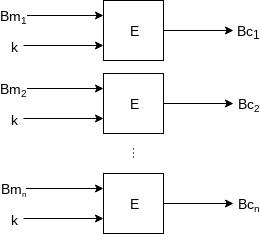
\includegraphics[width=0.7\linewidth]{diagramas/modo_ecb.png}
      \caption{Cifrado.}
    \end{center}
  \end{subfigure}
  \begin{subfigure}{0.45\textwidth}
    \begin{center}
      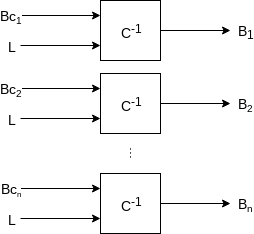
\includegraphics[width=0.7\linewidth]{diagramas/modo_ecb_inverso.png}
      \caption{Descifrado.}
    \end{center}
  \end{subfigure}
  \caption{\Gls{gl:modo_de_operacion} \gls{gl:ecb}.}
  \label{figura:ecb}
\end{figure}

\begin{pseudocodigo}[%
    caption={\Gls{gl:modo_de_operacion} \gls{gl:ecb}, cifrado.}%
  ]
  entrada: llave $ k $; bloques de mensaje $ Bm_1, Bm_2 \dots Bm_n $.
  salida:  bloques de mensaje cifrado $ Bc_1, Bc_2 \dots Bc_n $.
  inicio
    para_todo $Bm$
      $Bc_i$ $\gets$ E_k($Bm_i$)
    fin
    regresar $Bc$
  fin
\end{pseudocodigo}

\begin{pseudocodigo}[%
    caption={\Gls{gl:modo_de_operacion} \gls{gl:ecb}, descifrado.}%
  ]
  entrada: llave $ k $; bloques de mensaje cifrado $ Bc_1, Bc_2 \dots Bc_n $.
  salida:  bloques de mensaje original $ B_1, B_2 \dots B_n $.
  inicio
    para_todo $Bc$
      $Bm_i$ $\gets$ $D_k$($Bc_i$)
    fin
    regresar $Bm$
  fin
\end{pseudocodigo}
